% ============================================================
% Báo cáo môn học Xử lý ảnh — Tăng cường ảnh sử dụng bộ lọc
% bảo toàn cạnh (Clustering Filter)
% Tái tạo từ file Nhom_21_Bao_Cao-1.pdf
% Biên dịch: pdflatex main.tex (chạy 2 lần để có mục lục)
% ============================================================
\documentclass[a4paper]{report}

% Font 13pt + giãn dòng 1.3 — đo chính xác từ PDF gốc (baseline 20.28pt)
\usepackage[fontsize=13pt]{scrextend}
\linespread{1.3}

\usepackage[utf8]{inputenc}
\usepackage[T5]{fontenc}
\usepackage[vietnamese]{babel}

\usepackage{amsmath,amssymb}
\usepackage{graphicx}
% Lề đo từ bản gốc: trái 30mm, phải 20mm, baseline đầu tiên tại 82.3bp từ mép trên
% bottom=29.98mm: baseline cuối bản gốc tại 756.9bp — bottom=3cm thiếu 0.05bp,
% bottom=2.95cm lại dư (cho phép 758.3 → sai pagination); footskip giữ số trang ở 786.7
\usepackage[a4paper,top=2.5cm,bottom=29.98mm,left=3cm,right=2cm,footskip=29.9pt]{geometry}
\usepackage{xcolor}
\usepackage{listings}
\usepackage[font=small]{caption} % caption bản gốc dùng cỡ small (11.9pt)
% Gap caption→nội dung sau figure của bản gốc lớn hơn mặc định ~9pt (đo 46.3bp
% so với 37.2bp mặc định), nén được ~2.4pt ở trang chật
\captionsetup{belowskip=8.4pt minus 2.4pt}
\usepackage{multirow}
\usepackage{enumitem}
\usepackage[titles]{tocloft} % mục lục dạng "Chương N ..." như bản gốc
\usepackage{tikz} % vẽ bìa theo toạ độ tuyệt đối đo từ bản gốc
\usepackage{hyperref} % giữ kiểu khung đỏ/xanh quanh link như bản gốc

% Đoạn văn bản gốc: không thụt đầu dòng, cách đoạn 5.1pt (đo từ PDF)
\setlength{\parindent}{0pt}
\setlength{\parskip}{5.1pt}


% Itemize khớp bản gốc: gap vào list 17.35pt (topsep+partopsep+parskip),
% gap ra list 15.45pt (topsep+parskip) — đo p9 (begin 37.5) và p7 (end 35.6)
\setlist[itemize]{topsep=10.35pt plus 3pt minus 6.5pt,
    partopsep=1.9pt plus 1pt minus 1pt,
    itemsep=9.93pt plus 2.2pt minus 1.4pt, parsep=0pt}

% Khoảng cách quanh figure: bản gốc không nén được (không có minus glue) —
% nếu cho shrink, trang 16 sẽ nhồi thêm 1 dòng sai với bản gốc
\setlength{\intextsep}{14.08pt plus 4.34pt}
\setlength{\textfloatsep}{21.68pt plus 2.17pt}

% Mục lục: "Chương 1 <tên>" với tên bắt đầu tại 69.46pt; section thụt 15.06pt
\renewcommand{\cftchappresnum}{\chaptername\ }
\setlength{\cftchapnumwidth}{69.46pt}
\setlength{\cftsecindent}{15.06pt}
\setlength{\cftsecnumwidth}{22.98pt}
\setlength{\cftbeforechapskip}{10.04pt}

% Không cho dòng đầu tiên của một đoạn nằm cuối trang (giải thích các điểm
% ngắt trang của bản gốc tại cuối chương 1 và sau Hình 3.3)
\clubpenalty=10000

% Heading dùng cơ chế chuẩn của report (giữ nguyên \addvspace semantics —
% quan trọng cho khoảng cách sau float; không dùng titlesec vì titlesec
% cộng thêm \parskip và không gộp glue)
\makeatletter
% Section bản gốc cỡ \large (14.95pt), không phải \Large mặc định.
% Before-skip = 3.5ex − parskip (TeX tự cộng parskip khi heading bắt đầu
% paragraph mới; bản gốc tổng gap đo được 44.0bp tương ứng giá trị này)
% Heading section bản gốc: font 14.95pt nhưng baselineskip 21.2pt (đo từ
% vị trí heading ngay sau tên chương — không có before-skip ở đó)
\renewcommand\section{\@startsection{section}{1}{\z@}%
    {-17.62pt \@plus -5.89pt \@minus -1.18pt}%
    {2.3ex \@plus .2ex}%
    {\normalfont\fontsize{14.95pt}{16.31pt}\selectfont\bfseries}}% 16.31×1.3 = 21.2pt
% Chapter có số: "Chương N" cỡ \huge (26.96pt), tên chương \LARGE (22.46pt)
\def\@makechapterhead#1{%
  \vspace*{-9.9\p@}%
  {\parindent \z@ \raggedright \normalfont
    \ifnum \c@secnumdepth >\m@ne
        \huge\bfseries \@chapapp\space \thechapter
        \par\nobreak
        \vskip 3.1\p@
    \fi
    \interlinepenalty\@M
    \LARGE \bfseries #1\par\nobreak
    \vskip 2.8\p@
  }}
% Chapter không số: \Huge cho "Mục lục" (sau TOC chuyển sang \LARGE — bản gốc
% dùng hai cỡ khác nhau cho hai nhóm heading này)
\def\@makeschapterhead#1{%
  \vspace*{22.9\p@}%
  {\parindent \z@ \raggedright \normalfont
    \interlinepenalty\@M
    \Huge \bfseries  #1\par\nobreak
    \vskip 39.9\p@
  }}
\makeatother

\graphicspath{{images/}}

% ---- Kiểu code Python giống bản gốc (nền xám, số dòng bên trái) ----
\definecolor{codebg}{rgb}{0.949,0.949,0.9216} % màu nền đo từ bản gốc
\definecolor{codekw}{rgb}{0.0,0.35,0.75}
\definecolor{codestr}{rgb}{0.8,0.1,0.1}
\definecolor{codecmt}{rgb}{0.45,0.45,0.45}
\lstset{
    language=Python,
    backgroundcolor=\color{codebg},
    basicstyle=\ttfamily\small,
    keywordstyle=\color{codekw}\bfseries,
    stringstyle=\color{codestr},
    commentstyle=\color{codecmt},
    numbers=left,
    numberstyle=\small\color{codecmt},
    numbersep=8pt,
    breaklines=true,
    showstringspaces=false,
    % bản gốc: ký tự code giữ bề rộng tự nhiên của font (không giãn cột cứng)
    columns=fullflexible,
    keepspaces=true,
    % đo từ bản gốc (trang 10: text→nền code 11.5bp trừ parskip); bản gốc
    % không nén skip này — độ co của trang nằm ở topsep của itemize
    aboveskip=5.7pt plus 2pt,
    belowskip=32.6pt plus 2pt minus 2.5pt,
    inputencoding=utf8,
    extendedchars=true,
}

\begin{document}

% ============================================================
% TRANG BÌA
% ============================================================
% Toàn bộ trang bìa đặt theo toạ độ tuyệt đối (đơn vị bp, gốc = góc trên-trái
% trang) đo trực tiếp từ vector của PDF gốc — khớp từng baseline.
\begin{titlepage}
\begin{tikzpicture}[remember picture, overlay,
    every node/.style={inner sep=0pt, outer sep=0pt}]
    % Gốc toạ độ: góc trên-trái trang, trục y hướng xuống
    \coordinate (NW) at (current page.north west);
    % Khung đôi: ngoài dày 3bp, trong mảnh 1bp (toạ độ path đo từ bản gốc)
    \draw[line width=2.99bp]
        ([shift={(70.863bp,-70.866bp)}]NW) rectangle ([shift={(552.759bp,-771.033bp)}]NW);
    \draw[line width=1bp]
        ([shift={(75.115bp,-75.118bp)}]NW) rectangle ([shift={(548.507bp,-766.781bp)}]NW);
    % Logo: bbox (266.46, 156.02) – (357.15, 246.70)
    \node[anchor=north west] at ([shift={(266.457bp,-156.015bp)}]NW)
        {
\includegraphics[width=90.689bp]{logo_uet}};
    % Các dòng căn giữa theo tâm khung (x = 311.81bp), neo tại baseline
    \node[anchor=base] at ([shift={(311.81bp,-103.9bp)}]NW)  {\bfseries ĐẠI HỌC QUỐC GIA HÀ NỘI};
    \node[anchor=base] at ([shift={(311.81bp,-124.1bp)}]NW)  {\bfseries TRƯỜNG ĐẠI HỌC CÔNG NGHỆ};
    \node[anchor=base] at ([shift={(311.81bp,-323.6bp)}]NW)  {\bfseries BÁO CÁO MÔN HỌC};
    \node[anchor=base] at ([shift={(311.81bp,-343.8bp)}]NW)  {\bfseries XỬ LÝ ẢNH};
    \node[anchor=base] at ([shift={(311.81bp,-420.7bp)}]NW)  {\bfseries TĂNG CƯỜNG ẢNH SỬ DỤNG BỘ LỌC BẢO TOÀN CẠNH};
    \node[anchor=base] at ([shift={(311.81bp,-440.9bp)}]NW)  {\bfseries (CLUSTERING FILTER)};
    % Bảng thông tin: cột nhãn x=164.3bp, cột giá trị x=256.4bp
    \node[anchor=base west] at ([shift={(164.3bp,-516.0bp)}]NW) {Giảng viên:};
    \node[anchor=base west] at ([shift={(256.4bp,-516.0bp)}]NW) {PGS.TS. Lê Thanh Hà};
    \node[anchor=base west] at ([shift={(164.3bp,-536.2bp)}]NW) {Môn học:};
    \node[anchor=base west] at ([shift={(256.4bp,-536.2bp)}]NW) {Xử lý ảnh};
    \node[anchor=base west] at ([shift={(164.3bp,-556.4bp)}]NW) {Lớp học phần:};
    \node[anchor=base west] at ([shift={(256.4bp,-556.4bp)}]NW) {INT3404E 1};
    \node[anchor=base west] at ([shift={(164.3bp,-576.6bp)}]NW) {Sinh viên:};
    \node[anchor=base west] at ([shift={(256.4bp,-576.6bp)}]NW) {Hoàng Minh Quân - 22028019};
    \node[anchor=base west] at ([shift={(256.3bp,-596.8bp)}]NW) {Đặng Hoàng Minh Nghĩa - 22028054};
    \node[anchor=base] at ([shift={(311.81bp,-712.4bp)}]NW)  {\bfseries HÀ NỘI - 2025};
\end{tikzpicture}
\end{titlepage}

% ============================================================
% MỤC LỤC — trang mục lục không đánh số; Chương 1 bắt đầu = trang 1
% ============================================================
\pagestyle{empty}
% Bản gốc: các dòng trong mục lục cách nhau đúng 20.2bp (không có parskip)
\begingroup
\setlength{\parskip}{0pt}
\tableofcontents
\addcontentsline{toc}{chapter}{Mục lục}
\endgroup
\thispagestyle{empty}
\clearpage
\pagestyle{plain}
\pagenumbering{arabic}

% Từ đây các chapter không số (Đóng góp, Link Source code, Tài liệu tham khảo)
% dùng cỡ \LARGE như bản gốc (đo: 22.38pt, baseline 110.9bp)
\makeatletter
\def\@makeschapterhead#1{%
  \vspace*{-9.9\p@}%
  {\parindent \z@ \raggedright \normalfont
    \interlinepenalty\@M
    \LARGE \bfseries  #1\par\nobreak
    \vskip 2.7\p@
  }}
\makeatother

% ============================================================
% CHƯƠNG 1
% ============================================================
\chapter{Giới thiệu}

\section{Giới thiệu bài toán}

Trong lĩnh vực xử lý hình ảnh kỹ thuật số, vấn đề tăng cường chất lượng hình ảnh
(image enhancement) luôn là một thách thức cốt lõi, đặc biệt khi các chi tiết quan
trọng bị mất mát do hạn chế của thiết bị ghi nhận hoặc hiển thị. Dải động ở đây
đề cập đến khoảng cách giữa mức sáng tối nhất mà một hệ thống có thể xử lý,
thường dẫn đến tình trạng các vùng sáng bị ``washed out'' (mờ nhạt) hoặc vùng
tối trở nên phẳng lì, thiếu chiều sâu. Trong thực tế, hiện tượng này phổ biến trong
nhiếp ảnh hàng ngày -- chẳng hạn như khi chụp ảnh phong cảnh dưới ánh nắng
chói chang, các chi tiết trên bầu trời hoặc bóng râm có thể biến mất hoàn toàn,
khiến bức ảnh mất đi sức sống. Tương tự, trong lĩnh vực y tế, hình ảnh từ máy
quét MRI thường gặp phải vấn đề tương tự, nơi các cấu trúc giải phẫu tinh vi bị
che lấp, ảnh hưởng trực tiếp đến khả năng chẩn đoán chính xác của bác sĩ, có thể
dẫn đến sai sót trong điều trị (Hình \ref{fig:mri}).

\begin{figure}[htbp]
    \centering
    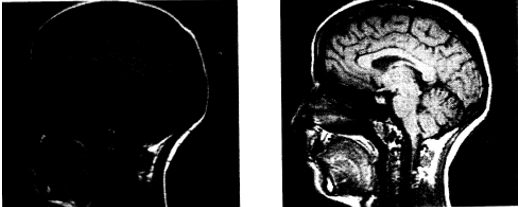
\includegraphics[width=\textwidth]{hinh1_1_mri}
    \caption{Hình ảnh từ máy quét MTI trước và sau khi được cải thiện chất lượng.}
    \label{fig:mri}
\end{figure}

Phương pháp truyền thống để khắc phục thường dựa vào việc trừ một phiên bản
lọc thông thấp khỏi hình ảnh gốc nhằm nhấn mạnh thành phần tần số cao, từ
đó khôi phục chi tiết. Tuy nhiên, cách tiếp cận này lại dễ dàng tạo ra các hiệu
ứng không mong muốn như ``halo'' -- những viền sáng hoặc tối giả tạo quanh các
cạnh biên, làm giảm tính tự nhiên và thẩm mỹ của hình ảnh (Hình \ref{fig:halo}). Chính
những hạn chế này đã thúc đẩy các nghiên cứu hướng tới các bộ lọc bảo toàn cạnh
(Edge-preserving filters), nhằm làm mịn hình ảnh mà vẫn giữ nguyên các biên giới
quan trọng, từ đó tạo ra một mask lý tưởng cho quá trình tăng cường.

\begin{figure}[htbp]
    \centering
    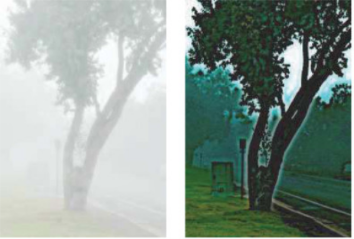
\includegraphics[width=\textwidth]{hinh1_2_halo}
    \caption{Hiệu ứng Halo (Xuất hiện vạch sáng rõ nét ở các cạnh vật thể).}
    \label{fig:halo}
\end{figure}

Bài báo ``Image Enhancement by Edge-Preserving Filtering''\cite{wong1994} của Yiu-fai Wong
(1994) chính là một đóng góp tiên phong trong hướng đi này, tập trung vào việc
sử dụng bộ lọc clustering để giải quyết vấn đề, mang lại kết quả vượt trội trong
việc nén dải động và tăng cường chi tiết mà không hy sinh tính chân thực. Kết
quả của nghiên cứu không chỉ nâng cao trải nghiệm thị giác trong giải trí mà còn
hỗ trợ đáng kể trong các lĩnh vực khoa học và y tế, nơi độ chính xác của hình ảnh
có thể quyết định sự thành bại.

\section{Tổng quan tài liệu}

Lĩnh vực tăng cường hình ảnh (image enhancement) đã thu hút sự quan tâm từ
sớm, tập trung vào việc khắc phục hạn chế dải động và cải thiện chi tiết mà không
làm méo mó cấu trúc cạnh biên. Các nghiên cứu ban đầu thường sử dụng kỹ thuật
lọc thông thấp truyền thống để tạo mask, nhưng dễ dẫn đến hiệu ứng halo không
mong muốn. Ví dụ, Schreiber\cite{schreiber1978} (1978) đã tổng quan các phương pháp xử lý hình
ảnh nhằm nâng cao chất lượng, nhấn mạnh vai trò của lọc tần số cao trong việc
khôi phục chi tiết bị mất trong các thiết bị hiển thị. Tương tự, Yule\cite{yule1967} (1967) khám
phá nguyên tắc tái tạo màu sắc, đề xuất các cách điều chỉnh dải động trong in ấn
và nhiếp ảnh, đặt nền tảng cho các kỹ thuật nén dải động sau này.

Trước năm 1994, một số công trình tiên phong đã hướng tới lọc bảo toàn cạnh
(edge-preserving smoothing) để giải quyết vấn đề trên. Nagao và Matsuyama\cite{nagao1979}
(1979) giới thiệu phương pháp lọc bảo toàn cấu trúc cạnh và giảm nhiễu, áp dụng
cho xử lý hình ảnh tự nhiên, trở thành nền tảng cho các mô hình sau. Perona và
Malik\cite{perona1990} (1990) đề xuất mô hình khuếch tán dị hướng (anisotropic diffusion), cho
phép làm mịn hình ảnh mà vẫn giữ nguyên cạnh biên, được áp dụng rộng rãi trong
phát hiện cạnh và tăng cường. Ngoài ra, Moore\cite{moore1992} (1992) sử dụng lưới điện trở bão
hòa để tạo mask trong tái tạo tông màu, truyền cảm hứng cho các phương pháp
lọc không tuyến tính, giúp tránh overshoot gần cạnh biên. Những nghiên cứu này
đã mở đường cho các cải tiến như clustering filter trong bài báo của Wong.

\section{Cơ sở lý thuyết}

Bài báo ``Image Processing for Quality Improvement''\cite{schreiber1978} của William F. Schreiber
(1978) là kết quả nghiên cứu nhằm mục tiêu kết nối kiến thức từ lĩnh vực nghệ
thuật đồ họa truyền thống (như nhiếp ảnh và in ấn) với các phương pháp xử lý hình
ảnh bằng máy tính, tập trung vào việc cải thiện chất lượng hình ảnh bằng cách
phân tích độ nhạy tương phản (contrast sensitivity), mối quan hệ giữa chiếu sáng
(illumination), phản xạ vật thể (reflectance), và độ sáng hình ảnh (luminance). Ở
nghiên cứu này, ông đề xuất các phương pháp lọc thích ứng (adaptive filtering)
khai thác hiện tượng tri giác và đặc tính vật lý của hệ thống hình ảnh, nhằm đạt
độ sắc nét cao đồng đều trên toàn thang độ sáng (tone scale) và các vùng hình
ảnh khác nhau, mà tránh hiệu ứng xấu như halo hoặc overshoot---các ý tưởng này
làm nền tảng cho các bộ lọc bảo toàn cạnh sau này, bao gồm công thức nền tảng
về bộ lọc bảo toàn cạnh trong bài báo gốc.

Giả sử $x_i$ là tọa độ pixel và $y_i$ là mức xám (gray level). Giá trị đầu ra $y$ tại vị trí $x$
được xác định bởi công thức lặp hội tụ sau:
% Riêng phương trình này bản gốc có khoảng cách trên 27.3pt (các display khác 13pt)
{\setlength{\abovedisplayskip}{22.9pt plus 2.6pt minus 2.6pt}%
\setlength{\belowdisplayskip}{11.8pt plus 2.6pt minus 2.6pt}%
\begin{equation}
    y = \frac{\sum_i y_i w_i e^{-\beta(y_i-y)^2}}{\sum_j w_j e^{-\beta(y_j-y)^2}}
    \label{eq:clustering}
\end{equation}}

\textbf{Trong đó:}

\begin{itemize}
    \item $w_i = e^{-\alpha\|x_i-x\|^2}$: Trọng số không gian, giảm dần theo khoảng cách từ tâm $x$.
          Tham số $\alpha$ quy định bán kính ảnh hưởng hiệu quả.
    \item $e^{-\beta(y_i-y)^2}$: Trọng số cường độ. Nó đóng vai trò như một hàm chọn lọc, chỉ cho
          phép các pixel có giá trị $y_i$ gần với giá trị $y$ được ưu tiên tham gia vào quá
          trình tính trung bình.
    \item $\beta = (2\sigma_y^2)^{-1}$: Tham số độ nhạy, được tính dựa trên phương sai cục bộ $\sigma_y^2$.
    \item
          \[
              \sigma_y^2 = \frac{\sum_i (y_i-\bar{y})^2 w_i}{\sum_i w_i}
          \]
          với
          \[
              \bar{y} = \frac{\sum_i y_i w_i}{\sum_i w_i}
          \]
\end{itemize}

Công thức \ref{eq:clustering} chính là một bước lặp của thuật toán Mean-Shift nổi tiếng (Co-
maniciu \& Meer, 2002\cite{comaniciu2002}). Mỗi lần lặp, giá trị $y$ được kéo về hướng ``mode'' (cụm
giá trị chiếm ưu thế nhất) trong phân bố xác suất hai chiều (vị trí không gian +
mức xám) của vùng lân cận. Khi lặp đủ số lần, $y$ sẽ dừng lại tại mode cục bộ $\rightarrow$
pixel được gán giá trị đại diện của cụm mà nó thuộc về.

Công thức có khả năng làm mịn mạnh:

\begin{itemize}
    \item Bên trong một vùng đồng nhất (ví dụ: bầu trời, bãi cỏ), các $y_i$ rất gần nhau
          $\rightarrow$ mode rất mạnh $\rightarrow$ $y$ nhanh chóng hội tụ về giá trị trung bình của vùng $\rightarrow$
          làm mịn cực tốt, gần như loại bỏ hoàn toàn texture nhỏ và nhiễu.
    \item Tại vùng gần biên mạnh (ví dụ: viền người quay phim), các pixel lân cận thuộc
          hai cụm hoàn toàn khác nhau (nền sáng và áo tối) $\rightarrow$ tồn tại hai mode riêng
          biệt $\rightarrow$ thuật toán sẽ ``nhảy'' pixel này sang đúng cụm mà nó thực sự thuộc về
          $\rightarrow$ biên được giữ nguyên vị trí và độ sắc nét, không bị mờ hay dịch chuyển.
\end{itemize}

Công thức có bước loại bỏ nhiễu hiệu quả: Một điểm nhiễu (rất sáng hoặc rất tối)
chỉ là một mode rất yếu (có rất ít pixel giống nó) $\rightarrow$ trọng số $e^{-\beta(y_i-y)^2}$ của nó gần
bằng 0 $\rightarrow$ hầu như không ảnh hưởng đến kết quả hội tụ $\rightarrow$ nhiễu bị triệt tiêu hoàn
toàn mà không cần bước tiền xử lý riêng.

Ngoài ra, tác giả đã phát triển công thức có khả năng thích nghi với quy mô:

\begin{itemize}
    \item Ở vùng phẳng ($\sigma_y$ nhỏ) $\rightarrow$ $\beta$ lớn $\rightarrow$ trọng số mức xám giảm rất nhanh với
          chênh lệch nhỏ $\rightarrow$ làm mịn mạnh hơn nữa.
    \item Ở vùng có cấu trúc ($\sigma_y$ lớn) $\rightarrow$ $\beta$ nhỏ $\rightarrow$ chấp nhận chênh lệch mức xám lớn
          hơn $\rightarrow$ bảo vệ chi tiết và cạnh.
\end{itemize}

% ============================================================
% CHƯƠNG 2
% ============================================================
\chapter{Phương pháp đề xuất}

Dựa trên bộ lọc Clustering Filter, quy trình tăng cường ảnh được thực hiện qua 6
bước như sau:

\section{Bước 1: Làm mượt ảnh (Smoothing)}

Trong bước đầu tiên của quy trình tăng cường hình ảnh, hình ảnh gốc $I$ được xử
lý thông qua bộ lọc clustering với tham số quy mô không gian $\alpha = 0.5$, áp dụng
theo cách đệ quy trong $k = 5$ lần lặp để tạo ra hình ảnh đã làm mịn $I_k$.

\begin{lstlisting}
    #Lap de quy 5 lan. Output lan truoc la Input lan sau.
    print("Step 1: Smoothing (Recursive filtering)...")
    Ii = I.copy()
    for k in range(5):
        print(f" Iteration {k+1}/5")
        Ii = clustering_filter_image(Ii, alpha=0.5, radius=3)
\end{lstlisting}

Quá trình này nhằm sản sinh một mask ban đầu, nơi các chi tiết cục bộ ở quy mô
nhỏ được làm mịn hóa một cách hiệu quả, đồng thời bảo toàn các cạnh biên nổi
bật giữa các cấu trúc lớn hơn, từ đó hỗ trợ việc tăng cường chi tiết sau này mà
không gây ra các artifact không mong muốn như hiệu ứng halo (viền sáng hoặc tối
giả tạo quanh cạnh). Tuy nhiên, bản chất của việc làm mịn ngụ ý rằng không phải
tất cả các tín hiệu hữu ích đều được giữ nguyên; ví dụ, các điểm sáng hoặc tối cô
lập có thể bị loại bỏ hoàn toàn bởi bộ lọc, các cạnh ở quy mô nhỏ hơn có thể bị
mờ đi, và các góc cạnh có thể bị bo tròn ở mức độ nhất định, đòi hỏi phải có sự
tinh chỉnh thêm ở các bước tiếp theo để khôi phục những yếu tố này.

\section{Bước 2: Tính sai khác (Difference)}

Ở bước thứ hai, ảnh sai khác được tính theo công thức $I_d = I - I_k$. Ảnh $I_d$ chứa
toàn bộ các thành phần tần số cao mà quá trình làm mịn ở bước 1 đã loại bỏ hoặc
làm suy giảm đáng kể, bao gồm:

\begin{itemize}
    \item Các chi tiết cục bộ ở quy mô nhỏ (fine details).
    \item Nhiễu (noise).
    \item Các điểm sáng/tối cô lập (bright/dark spots).
    \item Các cạnh quy mô nhỏ (small-scale edges).
    \item Sự sắc nét tại các góc cạnh (sharp corners) bị bo tròn trong quá trình lọc đệ
          quy.
\end{itemize}

\begin{lstlisting}
    print("Step 2: Difference Image...")
    Id = I - Ii
\end{lstlisting}

Theo tác giả, chính ảnh sai khác $I_d$ này lưu giữ lại những tín hiệu hữu ích đã bị
mất trong mask ban đầu $I_k$. Những tín hiệu này không thể bị loại bỏ hoàn toàn
trong quá trình tăng cường, bởi chúng đóng vai trò quan trọng trong việc tái tạo
độ chi tiết và độ tương phản tự nhiên của hình ảnh. Do đó, mục tiêu của các bước
tiếp theo (3 và 4) chính là xác định một cách thông minh những phần nào trong
$I_d$ thực sự mang tính ``chi tiết có ý nghĩa'' (ví dụ: góc cạnh, điểm sáng/tối thực) để
khôi phục lại vào mask, và phần nào chỉ là nhiễu hoặc artifact không cần thiết để
loại bỏ. Nhờ việc chọn lọc này, phương pháp của Wong tránh được hiện tượng halo
thường gặp trong kỹ thuật unsharp masking truyền thống, đồng thời vẫn đảm bảo
khả năng tăng cường chi tiết mạnh mẽ và tự nhiên.

\section{Bước 3: Thống kê cục bộ}

Ở bước thứ ba, để xác định chính xác phần nào của ảnh sai khác $I_d$ cần được khôi
phục vào mask, tác giả tính toán giá trị trung bình cục bộ $M(x)$ và phương sai
cục bộ $V(x)$ cho từng pixel trên ảnh $I_d$, sử dụng cửa sổ phân tích có kích thước
cố định $40\times40$ pixel. Việc này nhằm đánh giá mức độ biến thiên tự nhiên của tín
hiệu trong từng vùng cục bộ của ảnh sai khác.

\begin{lstlisting}
    print("Step 3: Local Mean & Variance (40x40 window)...")
    win_size = (40, 40)
    M = cv2.blur(Id, win_size) # Mean cuc bo
    # Tinh Variance cuc bo
    Id_sq = Id ** 2
    M_sq = cv2.blur(Id_sq, win_size)
    variance = M_sq - M**2
    V = np.sqrt(np.maximum(variance, 0))
\end{lstlisting}

Theo Wong, tại các vị trí chứa chi tiết có ý nghĩa thực sự --- chẳng hạn như các
góc cạnh sắc nét (sharp corners), điểm sáng hoặc tối cô lập (bright/dark spots),
hay các biên nhỏ bị làm mờ ở bước 1 --- giá trị $I_d(x)$ thường rất lớn so với độ lệch
chuẩn cục bộ (tức $|I_d(x) - M(x)|$ vượt đáng kể ngưỡng liên quan đến phương sai
$V(x)$). Ngược lại, ở những vùng phẳng hoặc chỉ chứa nhiễu ngẫu nhiên, sai lệch
này thường nằm trong khoảng biến thiên thông thường của khu vực lân cận. Do
đó, việc tính toán thống kê cục bộ đóng vai trò như một cơ chế phát hiện tự động:
nó phân biệt được đâu là ``tín hiệu chi tiết có cấu trúc'' (cần được giữ lại và khôi
phục) và đâu chỉ là ``biến động ngẫu nhiên'' (có thể bỏ qua). Kết quả của bước này
sẽ được sử dụng trực tiếp ở bước tiếp theo để đưa ra quyết định ngưỡng hóa thông
minh, từ đó hoàn thiện mask cuối cùng mà vẫn đảm bảo không tái tạo halo hay
overshoot --- một nhược điểm cố hữu của các kỹ thuật unsharp masking truyền
thống.

\section{Bước 4: Tạo mặt nạ (Mask Generation)}

Ở bước quan trọng nhất, mặt nạ hoàn chỉnh $I_m$ được xây dựng bằng cách khôi
phục có chọn lọc các tín hiệu từ ảnh sai khác $I_d$ vào mask ban đầu $I_k$, theo quy
tắc ngưỡng hóa sau:
\[
    I_m(x) =
    \begin{cases}
        I_k(x) & \text{nếu } |I_d(x) - M(x)| < 2.5\,V(x) \\
        I(x)   & \text{trường hợp còn lại}
    \end{cases}
\]

Ngưỡng $2.5\,V(x)$ (tương đương khoảng 2.5 lần độ lệch chuẩn cục bộ) đóng vai trò
như một bộ phân loại tự động thông minh:

\begin{itemize}
    \item Nếu độ lệch $|I_d(x) - M(x)|$ nhỏ hơn ngưỡng $\rightarrow$ biến động tại pixel đó chỉ nằm
          trong phạm vi biến thiên bình thường của vùng lân cận $\rightarrow$ được coi là nhiễu
          nền hoặc chi tiết không đáng kể $\rightarrow$ giữ nguyên giá trị đã làm mịn $I_k(x)$.
    \item Nếu độ lệch vượt quá ngưỡng $\rightarrow$ tín hiệu sai khác tại đó bất thường lớn so với
          vùng xung quanh $\rightarrow$ rất có khả năng là chi tiết cấu trúc thực sự (góc cạnh sắc
          nét, điểm sáng/tối cô lập, biên nhỏ bị làm mờ ở bước 1) $\rightarrow$ lấy trực tiếp giá
          trị từ ảnh gốc $I(x)$ để khôi phục hoàn toàn độ tương phản và độ sắc nét ban
          đầu.
\end{itemize}

\begin{lstlisting}
    print("Step 4: Creating Mask...")
    # Neu sai khac nho hon 2.5 lan do bien dong -> La nhieu -> Lay anh muot
    # Neu sai khac lon -> La chi tiet quan trong -> Lay anh goc
    mask_condition = np.abs(Id - M) < (2.5 * V)
    Im = np.where(mask_condition, Ii, I)
\end{lstlisting}

Nhờ cơ chế ngưỡng hóa thích nghi dựa hoàn toàn trên thống kê cục bộ này, phương
pháp của Wong đạt được hai mục tiêu đồng thời:

\begin{itemize}
    \item Giữ được độ mịn của mask ở những vùng chứa chi tiết nhỏ và nhiễu (tránh
          hiện tượng halo/overshoot thường gặp trong unsharp masking truyền thống).
    \item Khôi phục triệt để các chi tiết có ý nghĩa cấu trúc mà bộ lọc clustering đã vô
          tình làm mất hoặc làm tròn ở bước 1.
\end{itemize}

Kết quả là mặt nạ $I_m$ vừa mượt ở các vùng cần mượt, vừa có độ sắc nét cần thiết
tại các biên và chi tiết quan trọng --- điều kiện lý tưởng để thực hiện phép trừ ở
bước tiếp theo mà vẫn cho ra hình ảnh tăng cường tự nhiên, không artifact.

\section{Bước 5: Tăng cường (Enhancement)}

Sau khi đã có mặt nạ hoàn chỉnh $I_m$ --- vừa mượt ở các vùng chi tiết nhỏ, vừa giữ
được độ sắc nét tại các biên và cấu trúc quan trọng --- bước thứ năm thực hiện
phép tăng cường chi tiết bằng cách trừ một phần mặt nạ này khỏi ảnh gốc:
\[
    I_o = I - s \cdot I_m \quad \text{với} \quad s = 0.5
\]

Hệ số $s = 0.5$ được chọn nhằm kiểm soát cường độ tăng cường:

\begin{itemize}
    \item Giá trị $s$ càng lớn $\rightarrow$ độ tương phản cục bộ (đặc biệt ở vùng tần số cao) càng
          được nhấn mạnh mạnh mẽ hơn.
    \item Giá trị $s = 0.5$ là mức cân bằng thực nghiệm mà Wong thấy cho kết quả tự
          nhiên nhất trên nhiều loại ảnh thực tế, tránh hiện tượng tăng cường quá mức
          dẫn đến nhiễu bị khuếch đại hoặc xuất hiện viền giả.
\end{itemize}

\begin{lstlisting}
    print("Step 5: Enhancement calculation...")
    s = 0.5
    Io = I - s * Im
\end{lstlisting}

Về bản chất, phép trừ này tương tự kỹ thuật unsharp masking cổ điển ($I_{enhanced} =
I + \lambda(I - I_{blurred})$), nhưng nhờ mặt nạ $I_m$ đã được tinh chỉnh thông minh ở các bước
trước (bảo toàn cạnh, khôi phục góc và điểm sáng/tối), quá trình tăng cường của
Wong đạt được hai ưu điểm vượt trội:

Chi tiết được nâng cao rõ rệt trên toàn ảnh (áo, cỏ, nền trong ảnh Cameraman;
cấu trúc giải phẫu trong ảnh MRI). Không xuất hiện hiệu ứng halo hoặc overshoot
quanh các cạnh mạnh --- nhược điểm cố hữu của unsharp masking truyền thống
và của các phương pháp sử dụng mặt nạ low-pass đơn thuần.

Kết quả sau bước 5 là ảnh $I_o$ có dải động bị nén nhẹ và phân bố độ sáng chưa tối
ưu (thường bị dịch chuyển và thu hẹp histogram), do đó cần bước cuối cùng để
đưa ảnh về phạm vi hiển thị đầy đủ và đẹp mắt nhất.

\section{Bước 6: Kéo dãn tương phản (Rescaling)}

Sau khi đã thu được ảnh tăng cường $I_o = I - s \cdot I_m$, histogram của $I_o$ thường bị dịch
chuyển và thu hẹp lại so với ảnh gốc (do phép trừ mặt nạ đã làm giảm thành phần
tần số thấp, đồng thời nén một phần dải động). Để đưa ảnh về phạm vi hiển thị
tối ưu và khai thác hết khả năng của thiết bị xuất (màn hình, máy in hoặc định
dạng lưu trữ), bước cuối cùng thực hiện chuẩn hóa tuyến tính dựa trên thống kê
toàn cục của chính $I_o$:

\begin{itemize}
    \item Tính trung bình toàn ảnh $m = \mathrm{mean}(I_o)$
    \item Tính độ lệch chuẩn toàn ảnh $v = \sqrt{\mathrm{var}(I_o)}$
    \item Ánh xạ tuyến tính toàn bộ giá trị của $I_o$ sao cho khoảng
          \[
              [m - 2.5v,\ m + 2.5v]
          \]
          được kéo giãn chính xác về khoảng giá trị đích (ví dụ: $[0,\,255]$ đối với ảnh 8-bit
          hoặc $[0,\,1]$ đối với ảnh thực).
\end{itemize}

\begin{lstlisting}
    m_o = np.mean(Io)
    v_o = np.std(Io)

    min_range = m_o - 2.5 * v_o
    max_range = m_o + 2.5 * v_o

    # Keo dan v 0-255
    Io_final = (Io - min_range) * (255.0 / (max_range - min_range))
    Io_final = np.clip(Io_final, 0, 255).astype(np.uint8)
\end{lstlisting}

Hệ số 2.5 được Wong lựa chọn thực nghiệm vì nó bao phủ khoảng 99\% năng lượng
tín hiệu trong phân bố gần chuẩn, đồng thời loại bỏ một phần rất nhỏ các giá
trị ngoại lai (outlier) cực đại/cực tiểu --- thường là nhiễu còn sót lại hoặc artifact
không đáng kể\cite{wong1994}.

% ============================================================
% CHƯƠNG 3
% ============================================================
\chapter{Kết quả thực nghiệm}

Thuật toán được cài đặt bằng ngôn ngữ Python sử dụng thư viện NumPy để tính
toán ma trận và OpenCV để xử lý ảnh.

\section{Dữ liệu thử nghiệm}

Mô hình được kiểm thử trên ảnh chuẩn ``Cameraman'' (256x256 pixel, Grayscale).

\begin{figure}[htbp]
    \centering
    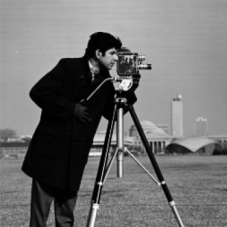
\includegraphics[width=181.42bp]{hinh3_1_cameraman}
    \caption{Ảnh gốc (I).}
    \label{fig:cameraman}
    % Bản gốc: gap caption→section sau figure NHỎ hơn gap caption→text 12pt
    % (hai giá trị mâu thuẫn, không thể đạt bằng một tham số toàn cục)
    \vspace{-12pt}
\end{figure}

\section{Kết quả}

Hình \ref{fig:ketqua} minh họa hiệu quả của thuật toán trên ảnh chuẩn ``Cameraman'':

\begin{itemize}
    \item Hình 1: Ảnh gốc -- chi tiết áo khoác, thảm cỏ và các tòa nhà nền bị mờ do dải
          động hạn chế và độ tương phản thấp.
    \item Hình 2: Mặt nạ cuối cùng $I_m$ -- quan sát rõ đặc tính của bộ lọc clustering
          kết hợp ngưỡng hóa thích nghi: vùng bầu trời và bãi cỏ cực kỳ mịn (gần như
          không còn texture nhỏ), trong khi viền áo, chân máy quay, đường viền khuôn
          mặt và các tòa nhà vẫn giữ được độ sắc nét rất cao, không bị bo tròn hay mờ
          đi. Điều này chứng tỏ mặt nạ đã loại bỏ hoàn toàn chi tiết không cần thiết
          nhưng bảo toàn xuất sắc các cấu trúc biên lớn và trung bình.
    \item Hình 3: Ảnh tăng cường cuối cùng -- chi tiết áo khoác (nếp gấp, nút áo), thảm
          cỏ, tóc và râu người quay phim trở nên rõ nét vượt trội so với ảnh gốc. Đặc
          biệt, không hề xuất hiện vệt trắng hoặc tối (halo/overshoot) quanh viền người
          và tripod dù độ tăng cường rất mạnh -- đây là ưu điểm nổi bật nhất so với
          unsharp masking truyền thống và các phương pháp sử dụng Gaussian blur
          làm mask.
\end{itemize}

\begin{figure}[htbp]
    \centering
    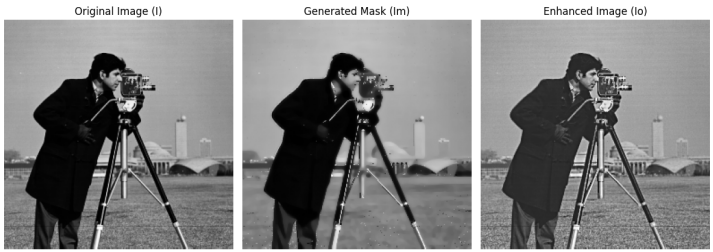
\includegraphics[width=\textwidth]{hinh3_2_ketqua}
    \caption{Kết quả sau khi thực hiện thuật toán trên ảnh gốc.}
    \label{fig:ketqua}
    % Như Hình 3.1: bản gốc dùng gap caption→section nhỏ hơn caption→text
    \vspace{-17.3pt}
\end{figure}

\section{Phân tích kết quả so với các phương pháp khác}

Để đánh giá khách quan ưu thế của phương pháp đề xuất, nhóm đã so sánh trực
quan kết quả tăng cường với hai kỹ thuật phổ biến nhất thời điểm đó là Histogram
Equalization (HE) toàn cục và Contrast Limited Adaptive Histogram Equalization
(CLAHE).

Histogram Equalization (HE) là một kỹ thuật tăng cường tương phản cổ điển, hoạt
động bằng cách cân bằng phân bố histogram toàn cục của hình ảnh để phân tán
đều các mức xám từ 0 đến 255 (đối với ảnh 8-bit), từ đó tăng cường độ tương phản
tổng thể và làm nổi bật chi tiết ẩn.

CLAHE, một biến thể thích nghi của HE, cải tiến bằng cách thực hiện cân bằng
histogram cục bộ trên từng vùng nhỏ (tile) của hình ảnh, đồng thời áp dụng giới
hạn tương phản (clip limit) để ngăn chặn over-amplification. CLAHE thường được
sử dụng trong xử lý ảnh y khoa hoặc ảnh có chiếu sáng không đồng đều, giúp bảo
tồn tốt hơn chi tiết cục bộ so với HE toàn cục.

\begin{lstlisting}
def wong_enhancement_comparison(image_path=None, alpha=0.5, radius=3, smooth_iters=5):
    img = cv2.imread(image_path, cv2.IMREAD_GRAYSCALE)
    if img is None:
            raise FileNotFoundError(f"Khong tim thay anh tai: {image_path}")

    I = img.astype(np.float32)

    #HE & CLAHE
    he = cv2.equalizeHist(img)
    clahe = cv2.createCLAHE(clipLimit=2.0, tileGridSize=(8,8))
    clahe_img = clahe.apply(img)
\end{lstlisting}

Hình \ref{fig:sosanh} minh họa kết quả so sánh trên ảnh ``Cameraman'' giữa phương pháp đề
xuất của Wong (Proposed), HE, và CLAHE, so với ảnh gốc (Original).

\begin{figure}[htbp]
    \centering
    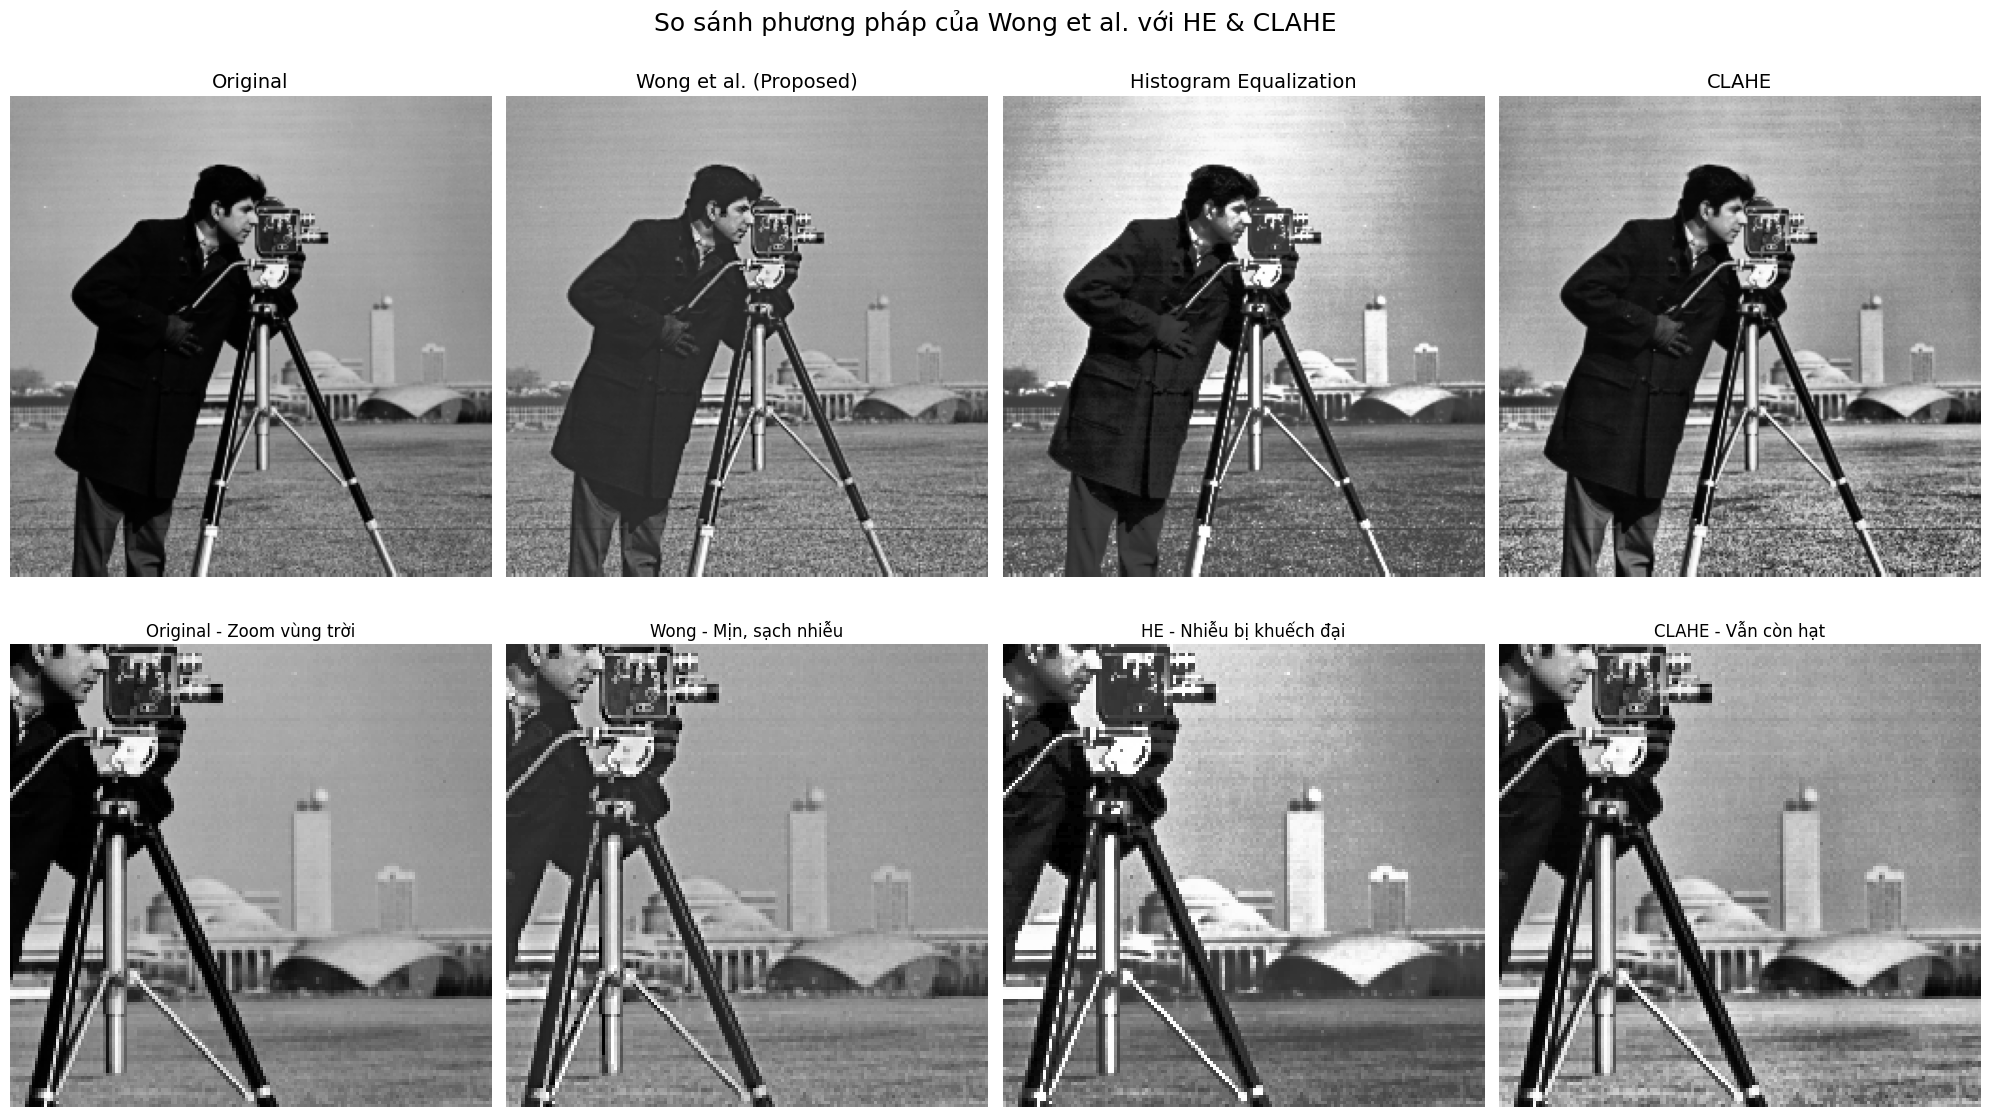
\includegraphics[width=\textwidth]{hinh3_3_sosanh}
    \caption{Kết quả so sánh các phương pháp.}
    \label{fig:sosanh}
\end{figure}

Quan sát tổng thể cho thấy:

\begin{itemize}
    \item Ảnh gốc (Original): Chi tiết trên áo khoác, thảm cỏ và tòa nhà nền bị mờ
          nhạt do dải động hạn chế và độ tương phản thấp.
    \item Phương pháp Wong (Proposed): Tăng cường rõ rệt chi tiết áo, cỏ, và khuôn
          mặt mà vẫn giữ quan hệ sáng-tối tự nhiên giữa các vùng lớn. Không xuất hiện
          halo quanh viền người quay phim hoặc chân máy, và vùng bầu trời mịn màng,
          không grainy. Trong zoom cận cảnh, cạnh biên mịn sạch, chi tiết nhỏ được
          khôi phục mà không bị over-sharpen.
    \item HE: Tăng cường tương phản mạnh nhưng dẫn đến over-saturation ở vùng sáng
          (bầu trời bị washed-out, tòa nhà nền mất chiều sâu) và nhiễu khuếch đại ở
          vùng tối (áo và cỏ trở nên grainy, nhiều artifact). Trong zoom, nhiều vùng bị
          nhiễu và quan hệ sáng-tối bị thay đổi không tự nhiên.
    \item CLAHE: Tốt hơn HE nhờ xử lý cục bộ, chi tiết áo và cỏ rõ nét hơn ảnh gốc,
          nhưng vẫn còn hạt (noise) ở vùng phẳng (bầu trời và cỏ) và over-contrast cục
          bộ ở một số cạnh (viền áo hơi halo nhẹ). Trong zoom, CLAHE giữ tốt chi tiết
          nhưng không mịn bằng Wong, và vẫn có hiện tượng ``vẫn còn hạt'' ở vùng tối.
\end{itemize}

Tổng thể, phương pháp Wong vượt trội ở khả năng tăng cường chi tiết đồng đều
mà không tạo artifact, đặc biệt ở các vùng chuyển tiếp cạnh biên, trong khi HE và
CLAHE thường làm thay đổi quá mức histogram dẫn đến mất cân bằng.

% ============================================================
% CHƯƠNG 4
% ============================================================
\chapter{Kết luận}

Bài báo ``Image Enhancement by Edge-Preserving Filtering'' của Yiu-fai Wong
(1994) đã đề xuất một quy trình tăng cường hình ảnh hoàn chỉnh, thông minh và
hiệu quả cao dựa trên việc khai thác triệt để đặc tính bảo toàn cạnh của bộ lọc
clustering. Khác biệt lớn nhất so với các phương pháp cổ điển (unsharp masking
truyền thống, Gaussian blur, hay histogram equalization) nằm ở khả năng tạo ra
mặt nạ thông minh: mặt nạ này không chỉ làm mịn các vùng chi tiết nhỏ và nhiễu
một cách mạnh mẽ, mà còn tự động nhận diện và khôi phục lại các cấu trúc quan
trọng như góc cạnh, điểm sáng/tối cô lập và biên nhỏ thông qua cơ chế ngưỡng
hóa thích nghi dựa trên thống kê cục bộ. Nhờ đó, thuật toán đạt được độ tăng
cường chi tiết rất mạnh, đồng đều trên toàn ảnh, đồng thời hoàn toàn loại bỏ hiện
tượng halo/overshoot -- vốn là nhược điểm cố hữu và khó khắc phục của hầu hết
các kỹ thuật tăng cường cùng thời kỳ.

Kết quả thực nghiệm trên cả ảnh cảnh thực tế (Cameraman) đã chứng minh tính
vượt trội rõ rệt: chi tiết được làm rõ đáng kể, quan hệ sáng-tối giữa các vùng lớn
được bảo tồn tự nhiên. Những đặc điểm này khiến phương pháp không chỉ có giá
trị học thuật mà còn rất thực tiễn, đặc biệt trong các ứng dụng yêu cầu chất lượng
hình ảnh cao như chẩn đoán y khoa, xử lý ảnh vệ tinh, và phục chế ảnh cũ.

Mặc dù được công bố từ năm 1994, ý tưởng cốt lõi của bài báo -- kết hợp lọc bảo
toàn cạnh với khôi phục chi tiết thích nghi -- vẫn là nền tảng cho rất nhiều thuật
toán hiện đại ngày nay (Như bilateral filter, guided filter, L0 smoothing, domain
transform,...). Một số hướng phát triển tiềm năng dựa trên phương pháp có thể kể
đến:

\begin{itemize}
    \item Tăng tốc độ tính toán bằng cách triển khai song song trên GPU hoặc sử dụng
          các biến thể nhanh của mean-shift/clustering (ví dụ: fast bilateral approxima-
          tion).
    \item Mở rộng sang không gian màu (RGB, Lab, HSV) hoặc xử lý ảnh màu đa kênh
          đồng thời.
    \item Ứng dụng trong video enhancement thời gian thực hoặc xử lý ảnh HDR.
\end{itemize}

Có thể nói kết quả của bài báo là một đóng góp tiên phong và bền vững trong lĩnh
vực xử lý ảnh số, đặt nền móng cho hàng loạt nghiên cứu tăng cường ảnh hiệu quả
cao sau này.

% ============================================================
% ĐÓNG GÓP THÀNH VIÊN
% ============================================================
\chapter*{Đóng góp các thành viên trong nhóm}
\addcontentsline{toc}{chapter}{Đóng góp thành viên}

% Bảng đo từ bản gốc: 3 cột tại x = 85.2 / 237.2 / 476.3 / 559.6bp;
% khoảng cách heading→bảng của bản gốc tương đương heading→text (26.2bp)
\vspace{12.8pt}
\begin{tabular}{|p{49.4mm}|p{80.1mm}|p{25.1mm}|}
\hline
\textbf{Sinh viên} & \textbf{Tác vụ thực hiện} & \textbf{Đóng góp (\%)} \\
\hline
\multirow{4}{*}{Đặng Hoàng Minh Nghĩa}
    & Nghiên cứu tài liệu                    & \multirow{4}{*}{50\%} \\
    & Thực hiện viết và điều chỉnh code      & \\
    & Thực hiện kiểm thử với ảnh thực tế     & \\
    & Làm slide                              & \\
\hline
\multirow{4}{*}{Hoàng Minh Quân}
    & Nghiên cứu tài liệu                    & \multirow{4}{*}{50\%} \\
    & Thực hiện viết và điều chỉnh code      & \\
    & Làm slide chính                        & \\
    & Viết báo cáo                           & \\
\hline
\end{tabular}

% ============================================================
% LINK SOURCE CODE
% ============================================================
\chapter*{Link Source code của nhóm}
\addcontentsline{toc}{chapter}{Link Source code}

Dưới đây là source code được nhóm trình bày lại. Do bài báo đã miêu tả rõ ràng
về ý tưởng xử lý nên nhóm đã tự code lại toàn bộ thuật toán được nêu trong bài
báo và không sử dụng AI, đồng thời mở rộng bằng cách so sánh trực quan kết quả
tăng cường với hai kỹ thuật phổ biến nhất thời điểm đó là Histogram Equalization
(HE) toàn cục và Contrast Limited Adaptive Histogram Equalization (CLAHE).

\textbf{Link Source code:} \href{https://colab.research.google.com/drive/17qr9Ct74zRE9zIkvhLAtKgD-q7CW0OxO?usp=sharing}{Source code}

% ============================================================
% TÀI LIỆU THAM KHẢO — nguyên văn trang 20 bản gốc (BibTeX plain style)
% ============================================================
\begin{thebibliography}{9}
% Khoảng cách đầu list và giữa các mục của bản gốc nhỏ hơn mặc định 2.8/2.4pt
% (babel/hyperref vô hiệu các hook chuẩn topsep/@openbib@code nên chỉnh tại env)
\vspace{-2.8pt}
\addtolength{\itemsep}{-2.4pt}
\addcontentsline{toc}{chapter}{Tài liệu tham khảo}

\bibitem{wong1994}
Yiu-fai Wong. Image enhancement by edge-preserving filtering. In \textit{Proceedings
of the IEEE International Conference on Image Processing}, volume 2, pages
522--524, Austin, TX, 1994. IEEE.

\bibitem{schreiber1978}
W. F. Schreiber. Image processing for quality improvement. \textit{Proceedings of the
IEEE}, 66(12):1640--1651, 1978.

\bibitem{yule1967}
John A. C. Yule. \textit{Principles of Color Reproduction: Applied to Photomechanical
Reproduction, Color Photography, and the Ink, Paper, and Other Related
Industries}. Wiley, 1967.

\bibitem{nagao1979}
M. Nagao and T. Matsuyama. Edge preserving smoothing. \textit{Computer Graphics
and Image Processing}, 9(4):394--407, 1979.

\bibitem{perona1990}
P. Perona and J. Malik. Scale-space and edge detection using anisotropic
diffusion. \textit{IEEE Transactions on Pattern Analysis and Machine Intelligence},
12(7):629--639, 1990.

\bibitem{moore1992}
Andrew John Moore. \textit{Spatial Filtering in Tone Reproduction and Vision}. Ph.d.
thesis, California Institute of Technology, 1992.

\bibitem{comaniciu2002}
Dorin Comaniciu and Peter Meer. Mean shift: A robust approach toward feature
space analysis. \textit{IEEE Transactions on Pattern Analysis and Machine Intelligence},
24(5):603--619, 2002.

\end{thebibliography}

\end{document}
